\documentclass[12pt,twocolumn,letterpaper]{article}

\usepackage{cvpr}
\usepackage{times}
\usepackage{epsfig}
\usepackage{graphicx}
\usepackage{amsmath}
\usepackage{amssymb}
\usepackage[breaklinks=true,bookmarks=false]{hyperref}
\usepackage{gensymb}
\usepackage{subcaption}

\cvprfinalcopy

\def\httilde{\mbox{\tt\raisebox{-.5ex}{\symbol{126}}}}


\setcounter{page}{1}
\begin{document}

\title{3D Perspective Effects on a Smart Phone}

\author{Jai Prakash\\
Carnegie Mellon University\\
Master of Science in Computer Vision\\
{\tt\small jprakash@andrew.cmu.edu}
\and
Jennifer Lake\\
Carnegie Mellon University\\
Master of Science in Computer Vision\\
{\tt\small jelake@andrew.cmu.edu}
}

\maketitle

\begin{abstract}
In this project, we aim to create a 3D perspective transformation on a smart phone screen that will give the illusion of screen having depth.  The user should feel as if they are looking into a long hallway, were objects can appear deeper and deeper into the hall. This is achieved by finding the three-dimensional vector between the user’s face and the center of the phone.  This was achieved by tracking the user’s face using the front-facing camera.  We also explored integrating this method with the smart phone's Internal Measurement Unit (IMU) in order to estimate the smart phone orientation. In both methods, Kalman filtering was used in order to create a more reliable vector prediction.
\end{abstract}

\section{Introduction}
\subsection{Motivation}
As mobile phones have evolved over the last twenty years, many of the major milestones have been in display improvements. Mobile phones have gone from very small, simple displays to larger and more colorful displays.  At the forefront of this evolution, there is a growing trend of three-dimensional displays. 

There are several benefits to having more 3D-like displays.  3D-like displays may help users interact with User Interfaces in a more intuitive way, such as using the phone movement itself as a command.  This can help when using the phones when wearing gloves, which do not allow the use of the touch screen.  In addition, 3D-like displays may help users navigate using 3D maps, which are more representative of the surroundings in urban areas. Finally, 3D-like displays would be a major boost to the gaming industry, which constantly strives to make more and more realistic games.  With perspective effects that mimic real-world perspective effects, the user would experience a more immersive gaming experience.

The holy grail of 3D perspective transforms is to be able to provide augmented reality to the user.  This would allow the user to use their smart phone to interact with the world around them in an intuitive manner, such as in figure 1.  We hope that some of the work in this project, may help in future projects striving towards this goal.


\begin{figure}[!htbp]
\centering
\begin{subfigure}{0.22\textwidth}
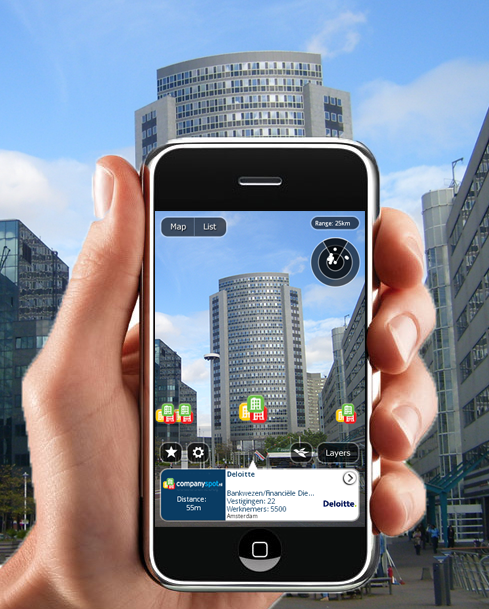
\includegraphics[height=35 mm]{AR_now}
\end{subfigure}
\begin{subfigure}{0.22\textwidth}
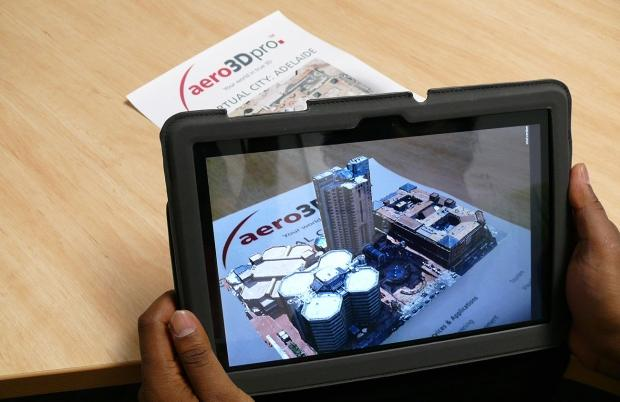
\includegraphics[height=25 mm]{AR_now1}
\end{subfigure}
\caption{Augemented reality in present smartphones}
\label{fig:arnow}
\end{figure}

\subsection{Background}

The change in appearance of an object when viewed from multiple viewpoints is known as parallax \cite{Szeliski}.  Parallax occurs due to the shift in perspective.  An example of the parallax effect is shown below \cite{Wikipedia}.

\begin{figure}[!htbp]
\centering
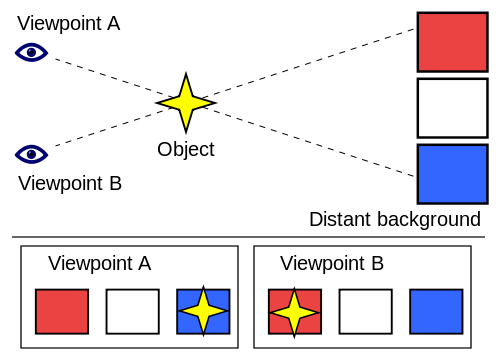
\includegraphics[height=30 mm]{parallax.png}
\caption{An example of the parallax effect.  The top of the figure shows the scene from above.  The bottom of the figure shows the views from each viewpoint.}
\end{figure}

There are three types of parallax effects: negative, zero, and positive parallax (figure 2) \cite{CSU}.  

\begin{figure}[!htbp]
\centering
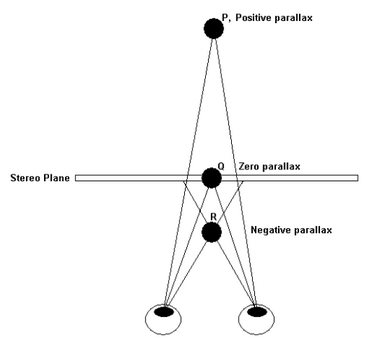
\includegraphics[height=35 mm]{NegPosParallax.png}
\caption{Example of positive, zero, and negative parallax}
\end{figure}

Positive parallax occurs when the user gets the impression of looking through the screen plane and this effect will be the focus of this project.  Negative parallax occurs when the user get the impression that objects are floating above the user screen and this effect will not be addressed in this project.  Zero parallax is the impression that the object lies on the screen and this conventional way of viewing objects on a screen.

\subsection{Related Work}
The trend of introducing of positive parallax effects into smart phones has been growing in the last few years.  In 2013, Apple introduced the positive parallax effect on their line of iPhones, which allows for a 3D-like feeling, by changing the position of the background wallpaper according to the orientation of the smart phone \cite{BusinessInsider}.  A year later, the Amazon Fire Phone introduced a full positive parallax effect, which was branded as "Dynamic Perspective" \cite{DigitalTrends}.  It is this type of effect that we aim to create in this project however, unlike the Amazon Fire Phone, we will be implementing this effect on simpler, standard smart phone hardware.

Prior to the growing trend in parallax effects in smart phones, the Microsoft Kinect was to estimate a person's pose and using that information, render a parallax effect on a television screen.  One interesting example of this is the Virtual Window, which has a television behind a false window and the landscape on the television changes based on the perspective of the user.  One major constraint of this type of system is that the perspective change only works for one user at a time.

In the future, we expect parallax effects to lead to Augemented Reality for smart phones.  This could allow users to seamlessly interact with the surrounding environment and could lead to new uses for smart phones.

\subsubsection{Virtual Window}
The Virtual Window works by using a Microsoft Kinect sensor, which projects a light pattern onto the user and uses an RGB-D camera to find the pose and 3-dimensional pose of the user \cite{Winscape}.  Using this information, the position of the user's head and eyes can be located using built-in tools in the Kinect API.  A high-resolution, high-quality image of an outdoor scene is then moved in order to simulate that the screen is in fact a window.  The image only needs to be shifted to the appropriate location because the images are taken from far away (see figure 4).

\begin{figure}[!htbp]
\centering
\begin{subfigure}{0.22\textwidth}
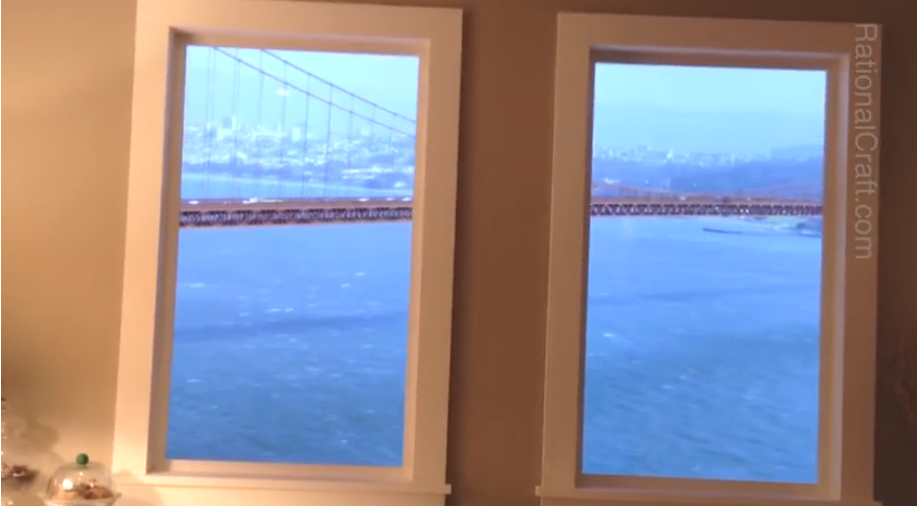
\includegraphics[width = 35 mm]{win1.png}
\end{subfigure}
\begin{subfigure}{0.22\textwidth}
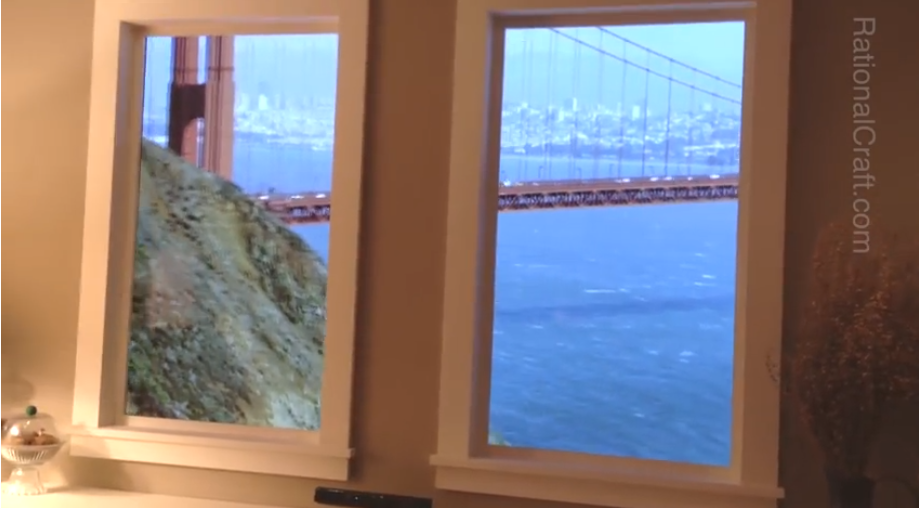
\includegraphics[width = 35 mm]{win2.png}
\end{subfigure}
\caption{Virtual Window from two different perspectives}
\end{figure}

\subsubsection{Amazon Fire Phone}
The Amazon Fire Phone uses four, front-facing camera's with wide 120 \degree viewing angles \cite{TechCrunch}.  This allows for at least two cameras to be able to locate the user's face, regardless of how the phone is held.  The face tracking works in low light as well, due to infrared light being used to illuminate the user's face.  By tracking the user's face, the vector between the phone and the user can be approximated and thereby the correct perspective transform can be computed and displayed.

\begin{figure}[!htbp]
\centering
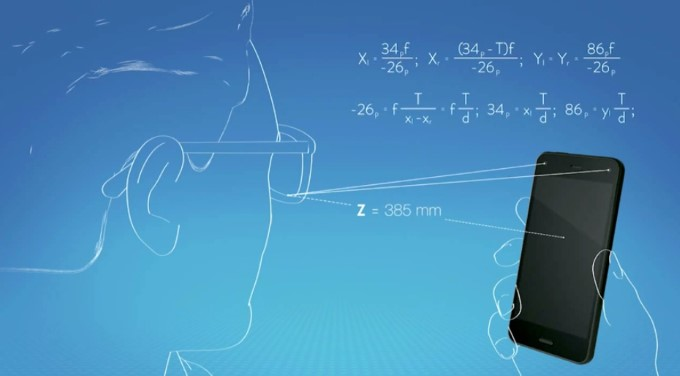
\includegraphics[height=35 mm]{dp.jpg}
\caption{Example of Amazon Fire Phone's Dynamic Perspective}
\end{figure}

\subsubsection{Augmented Reality}

The ultimate goal of estimating a phone's orientation with respect to the user is to be able to implement Augmented Reality (AR) into smart phones. The smart phone Augmented Reality can broadly be classified into two types:
\begin{itemize}
\item \textbf{Indirect AR} Figure \ref{fig:arnow} shows augmented reality applications in current smart phones. This gives the user a video see-through experience, as the view is from the camera's perspective.
\item \textbf{Direct AR} These are the systems that give a perspective from user's point of view and hence give more immersive experience than indirect AR system. The Microsoft Hololens and meta-glasses (Figure \ref{fig:directar}) are examples of direct AR systems. 
\end{itemize}


\begin{figure}[!htbp]
\centering
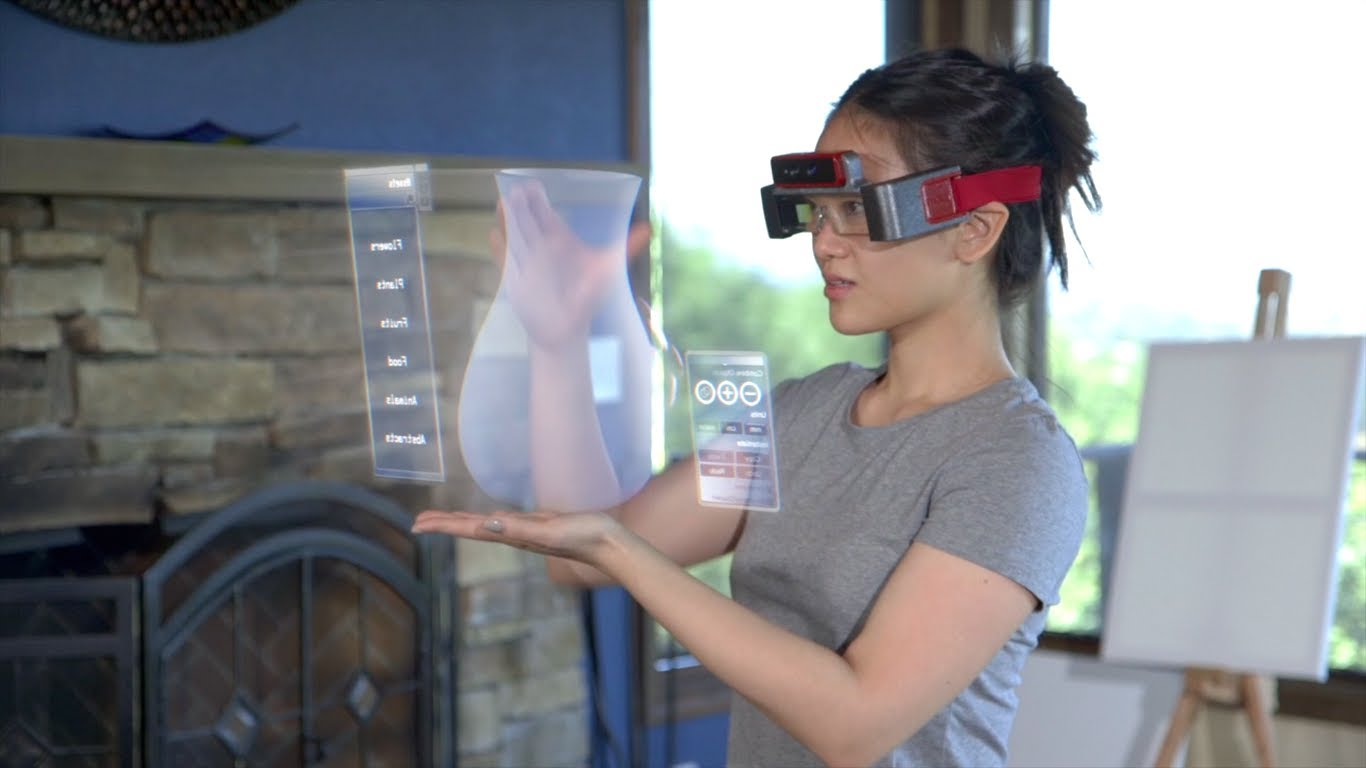
\includegraphics[height=30 mm]{mata}
\caption{Direct AR from Meta-glasses}
\label{fig:directar}
\end{figure}

The current direct AR systems are generally bulky and requires user to wear special glasses to use them. However, a direct AR system can be achieved in smart phones and tablets by using digital transparency \cite{jai}. Digital transparency system is shown in Figure \ref{fig:digitaltransparency}. This system tracks the eyes of the user and finds the angle which the tablet subtends at user's eye and crops the rear camera preview to the same angle to create a virtually transparent interface. This system gives a method to achieve direct AR on smart phones and tablets, thereby giving a more immersive \textbf{glass-see-through} experience than the conventional \textbf{video-see-through} experience.

\begin{figure}[!htbp]
\centering
\begin{subfigure}{0.22\textwidth}
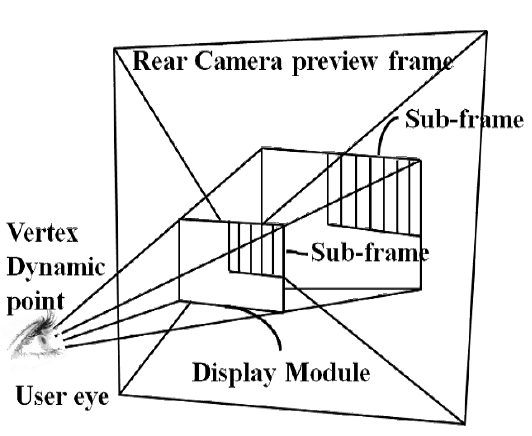
\includegraphics[height=30 mm]{transparenttablet}
\end{subfigure}
\begin{subfigure}{0.22\textwidth}
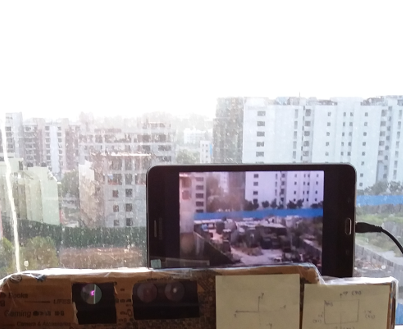
\includegraphics[height=30 mm]{transparenttablet1}
\end{subfigure}
\caption{Digital transparency using Kinect on Android tablet}
\label{fig:digitaltransparency}
\end{figure}

This method uses a Kinect sensor to track the accurate 3D position of the user with respect to tablet. The Kinect sensor makes the system bulkier and difficult to use in smart phones. So, in this project we are addressing another method to achieve digital transparency using just the front facing camera and attempting to integrate the inertial sensors. A complete hands-free digital transparency system is out of scope of this project. The main concentration is on creating a positive parallax effect which responds to the user's position with respect to the tablet.

\section{Method}
\begin{figure}[!htbp]
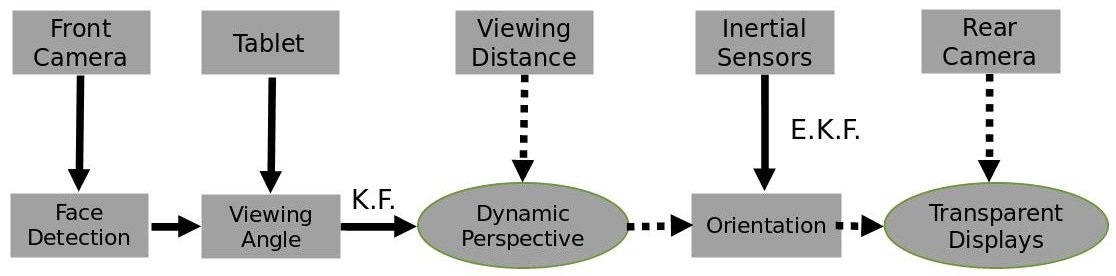
\includegraphics[scale=0.21]{block}
\caption{Block diagram of system}
\label{fig:blockdia}
\end{figure}

Creating a positive parallax effect involves finding the viewing angle of the user and rendering the graphical object depending on position of the user. This might involve one of three scenarios:
\begin{itemize}
\item Tablet is static and user moves
\item Tablet moves and user is static
\item Both tablet and the user can move
\end{itemize}

In order to limit the scope of the project, we have also placed a number of restrictions on how this systems is to be used.  We also assume the following restrictions:

\begin{itemize}
\item There are no drastic lighting changes
\item The user is not walking or running
\item The user is standing or sitting on a stationary surface.
\item The user and the tablet are moving smoothly and slowly
\item The tablet is held at a constant distance from the user's face.
\item There is only one user and the user is always in view of the front camera.
\item There are no other faces in the view of the front camera
\item The user is looking at the camera or very close to it
\item The user is an arm's length or less from the camera
\item The user's face is the primary object in the view of the camera
\end{itemize}

To find the motion and orientation of the phone, on-board inertial sensors can be deployed to find the orientation of the phone. A study on sensor fusion has been made to find the orientation of the phone.

The block diagram of the system is shown in the figure  \ref{fig:blockdia}. Solid arrow shows the algorithms implemented for this project. The dotted arrow parts are yet to be figured out to build a full-fledged digital transparency system. However, the main focus is only on creating the positive parallax effect.

To create this effect, we need to first track the position of user with respect to the tablet. In this project we assume that the distance of the eye from tablet is fixed (approximately 45-50 cm). This assumption fails to address the scale factor in dynamic perspective. Therefore we don't get zoom-in and zoom-out effect as we move forward and backward. Since the distance from the tablet is assumed to be constant, we use the viewing angle to render the user interface (UI) in 3D. The following sections describe the exact methods used in each step.

\subsection{3D Geometry of Problem}
In order to render a positive parallax effect, we must estimate the vector between the user and the phone, as shown in figure \ref{fig:vectors}.

\begin{figure}[!htbp]
\centering
\begin{subfigure}{0.22\textwidth}
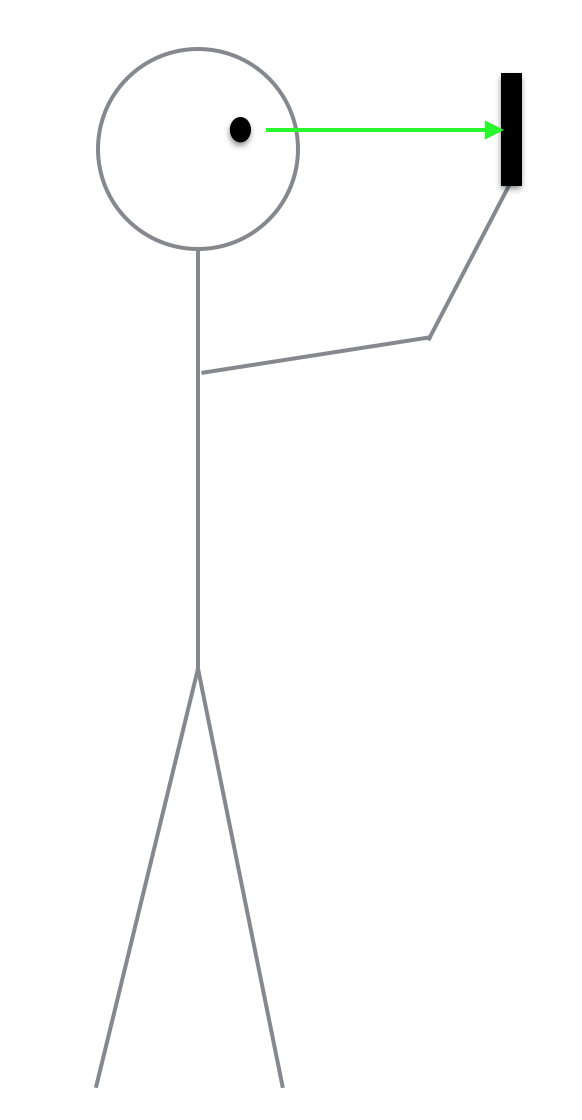
\includegraphics[height=30 mm]{vector1}
\end{subfigure}
\begin{subfigure}{0.22\textwidth}
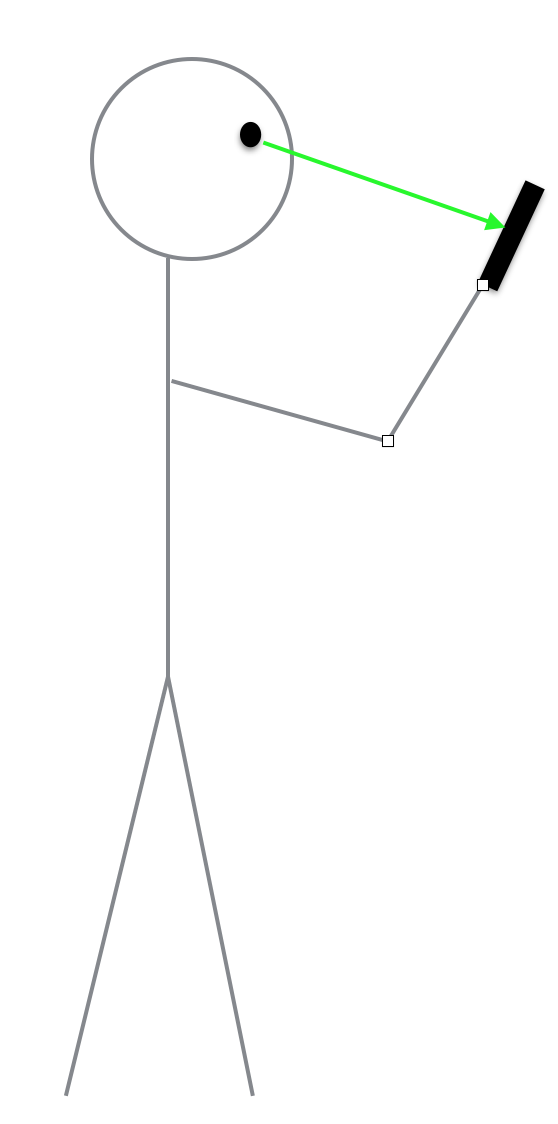
\includegraphics[height=30 mm]{vector2}
\end{subfigure}
\caption{Example of vectors to be found}
\label{fig:vectors}
\end{figure}

Normally, a user will hold a smart phone orthogonally to the vector between the user's eye and the principle point of the camera (figure \ref{fig:orthogonal}).  This is a natural position of the screen, since it is easiest to view from this angle and does not strain the eyes.   

\begin{figure}[!htbp]
\centering
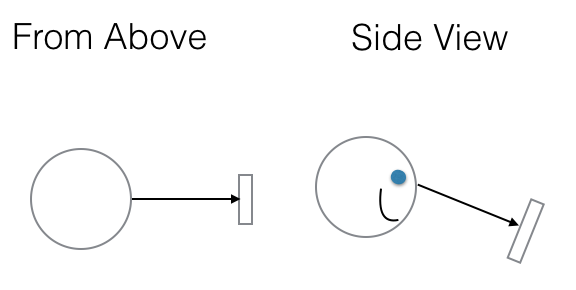
\includegraphics[height=30 mm]{conventional.png}
\caption{Conventional way of holding a smart phone}
\label{fig:orthogonal}
\end{figure}

However, it is possible for the user to hold the smart phone in an unconventional matter, such as in figure \ref{fig:unconventional}.

\begin{figure}[!htbp]
\centering
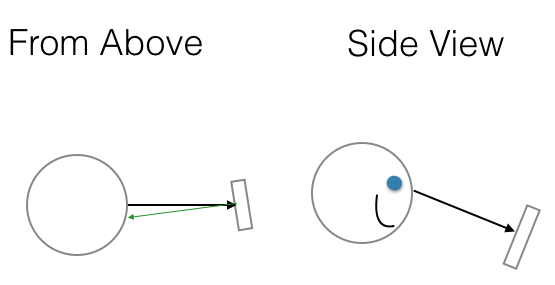
\includegraphics[height=30 mm]{unconventional.png}
\caption{Unconventional way of holding a smart phone.}
\label{fig:unconventional}
\end{figure}

In the majority of cases, users will be holding the tablet or smart phone in a conventional matter.  For that reason, we focused our efforts on that case.

\subsection{Finding viewing angle of user}
Since all the coordinates are in image frame of reference, the angle can be found by using the following equations. 
\begin{equation}
\theta_x = tan^{-1} \left( \frac{x_f - \frac{W}{2}}{f_x} \right)
\label{eqn:thetax}
\end{equation}
\begin{equation}
\theta_y = tan^{-1} \left( \frac{y_f - \frac{H}{2}}{f_y} \right)
\label{eqn:thetay}
\end{equation}

In equation \ref{eqn:thetax} and \ref{eqn:thetay}, $(x_f, y_f)$ is the location of the centroid of the user's face. Image size is $W \times H$. $f_x$ and $f_y$ are the focal length of the camera in pixels.

\begin{figure}[!htbp]
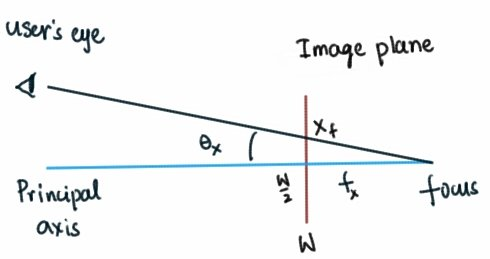
\includegraphics[scale=0.5]{view_angle}
\caption{The viewing angle of the user with respect to front camera on smart phone}
\label{fig:viewangle}
\end{figure}

Figure \ref{fig:viewangle} shows the viewing angle of the user. The view angle is the angle subtended by the user's position with the principal axis of the camera. The focal length of the camera is found by using camera calibration \cite{calibration}. 

\subsection{Face Detection}
The Viola-Jones algorithm was used for face detection because it is robust and fast \cite{Viola-Jones}.  The Viola-Jones algorithm has four main steps:

\begin{enumerate}
\item Compute Haar Features
\item Compute Integral Image
\item Use AdaBoost to Train Classifier
\item Cascade Classifiers
\end{enumerate}

In the first step, Haar features are computed.  Haar features represent simple structure present in human faces, such as darker eyes and lighter cheeks or a lighter nose and darker eyes.  These features are calculated at different orientations. An example of Haar features can be found in figure \ref{fig:Haar}.

\begin{figure}[!htbp]
\centering
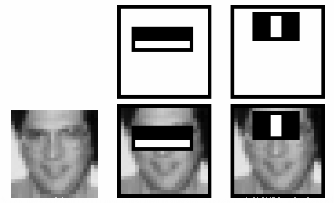
\includegraphics[scale=0.5]{haar}
\caption{An example of Haar features}
\label{fig:Haar}
\end{figure}

The integral image is then computed by summing the value of a pixel and all pixels to the left and above it.  This can be done in one pass if the integral image is calculated from the origin outward using equation \ref{eqn:integral}. This is done so that the Haar calculations, which are defined in equation \ref{eqn:haar} can be completed quickly.

\begin{multline}
\label{eqn:integral}
I(x,y) =  i(x,y) + I(x-1,y) 
\\+ I(x, y-1) - I(x-1, y-1)
\end{multline}


\textbf{\begin{equation}
\label{eqn:haar}
score = \sum{black pixels} - \sum{white pixels}
\end{equation}}

Using the Haar features, the AdaBoost algorithm is used to find the combination of weak classifiers that will yield a good result when combined.  The AdaBoost algorithm works by iteratively reweighing each training datapoint and calculating the boundary which yields the lowest error.  Datapoints which are previously misclassifed receive a higher weight and datapoints that were previously correctly classified receive a lower weight.  Using this iterative method, the combination of weak classifiers (the Haar features) can be combined to find faces.

The final step is to cascade the classifiers.  This is an optimization step where each Haar feature is ranked descending by how well they can identify a face.  This allows a quicker response during test time.
    
\subsection{Inertial Measurement Unit}
An Inertial Measurement Unit (IMU), is a sensor that features a triad of accelerometers and a triad of gyroscopes.  In cell phones, the IMU also typically features a magnetometer. 

\subsection{Kalman Filter}
The face detection using the cascade classifier is subject to jitter due to noise in the scene. The face detection sometimes fails because of various reasons like change is lighting conditions, change in expression of the face etc. This detection might cause jitter in the rendering. In order to avoid the jitter, we need to smooth the face detection and handle the no-detection case. The Kalman filter \cite{kalman}, can handle statistical uncertainties and other accuracies and produce results that are more accurate than a single measurement.

The Kalman filter models the uncertainties  in the states of position and velocities. The model alone is sufficient to predict the future uncertainties without remembering the past readings. which means that we can predict the state by knowing the parameters of the current state. Once the new reading arrive, the parameters of the model is updated.

\begin{figure}
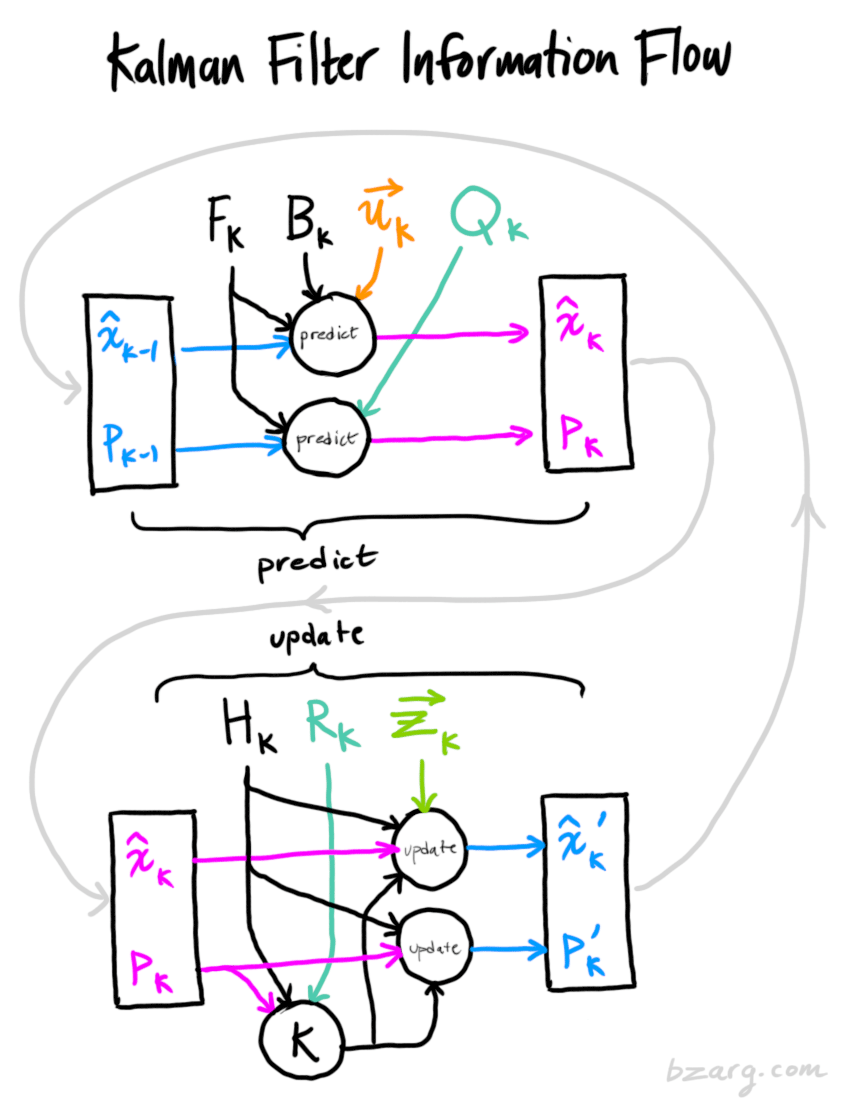
\includegraphics[scale=0.3]{kalflow}
\caption{Diagram showing the update in Kalman filter\\ credits: [13]}
\end{figure}

The prediction step is given by the equation
\begin{equation}
\hat{x_k} = \mathbf{F_k} \hat{x}_{k-1} + \mathbf{B_k} \vec{u_k}
\label{eqn:stateestimate}
\end{equation}
\begin{equation}
\mathbf{P_k} = \mathbf{F_k} \mathbf{P_{k-1}} \mathbf{F_k}^T + \mathbf{Q_k}
\label{eqn:estimatecovariance}
\end{equation}

Equation \ref{eqn:stateestimate} is called the state estimate (a priori) equation. And equation \ref{eqn:estimatecovariance} is called the estimate (a priori) covariance. The significance of each variable is as follows:
\begin{itemize}
\item $\mathbf{F_k}$ is the state transition model which is applied to the previous state $\hat{x}_{k−1}$
\item $\mathbf{B_k}$ is the control-input model which is applied to the control vector $\vec{u}_k$
\item $\mathbf{P_k}$ error covariance matrix (a measure of the estimated accuracy of the state estimate)
\item $\mathbf{Q_k}$ the covariance of the process noise
\end{itemize}

Moving on to the update step, once we get the readings from the actual scenario, we need to update the model to update our belief about the scene. The update equations are given as
\begin{equation}
\label{eqn:kalmangain}
\mathbf{K'} = \mathbf{P_k} \mathbf{H_k}^T \left( \mathbf{H_k} \mathbf{P_k} \mathbf{H_k}^T + \mathbf{R_k} \right)^{-1}
\end{equation}

\begin{equation}
\hat{x'}_k = \hat{x}_k + \mathbf{K'} \left( \vec{z}_k - \mathbf{H_k} \hat{x}_k \right)
\label{eqn:posterioristateestimate}
\end{equation}

\begin{equation}
\mathbf{P'_k} = \mathbf{P_k} - \mathbf{K'}  \mathbf{H_k} \mathbf{P_k}
\label{eqn:posterioriestimatecovariance}
\end{equation}

where,
$$ \vec{z}_k = \mathbf{H_k} \hat{x}_k + \vec{v}_k$$
$$ \vec{v}_k \approx \mathcal{N}(0, \mathbf{R_k})$$

The equation \ref{eqn:kalmangain} is called the Kalman gain of the filter. The equation \ref{eqn:posterioristateestimate} is the updated (a posteriori) state estimation of the filter. And the equation \ref{eqn:posterioriestimatecovariance} is known as the updated (a posteriori) state covariance equation. The variables used in these equations are described below:

\begin{itemize}
\item $\mathbf{H_k}$ is the observation model which maps the true state space into the observed space
\item $\vec{v}_k$ is the observation noise
\item $\mathbf{R_k}$ is the covariance of observation noise which is assumed to be zero mean Gaussian white noise
\end{itemize}

After applying Kalman filter, the face detection becomes continuous and smooth to be used for positive parallax.
\subsection{Extended Kalman Filter}
The Extended Kalman Filter is built upon the same principles as the Kalman filter in the previous section \cite{Maria}.  The main difference is the dynamics of the system can be non-linear and may be represented by differentiable functions instead.  The state transition is now represented by equation \ref{eqn:ekf-state}.  The observation model is now represented by equation \ref{eqn:ekf-obs}.

\begin{equation}
x_k = f(x_{k-1}, u_k) + w_{k-1}
\label{eqn:ekf-state}
\end{equation}

\begin{equation}
z_k = h(x_k) + v_k
\label{eqn:ekf-obs}
\end{equation}

The prediction stage then computes the predicted state estimate \ref{eqn:pred-state} and the predicted covariance estimate \ref{eqn:pred-cov}.

\begin{equation}
\hat{x}_{k|k-1} = f(\hat{x}_{k-1}, u_k)
\label{eqn:pred-state}
\end{equation}

\begin{equation}
P_{k|k-1} = F_kP_{k-1|k-1}F_k^T + Q_k
\label{eqn:pred-cov}
\end{equation}

The state transition and observation matrices are shown in \ref{eqn:ekf-F} and \ref{eqn:ekf-H}.

\begin{equation}
\hat{F}_{k|k-1} = \frac{\delta f}{\delta x}\Bigr|_{\hat{x}_{k-1|k-1}, u_{k-1}}
\label{eqn:ekf-F}
\end{equation}

\begin{equation}
H_{k} = \frac{\delta h}{\delta x}\Bigr|_{\hat{x}_{k|k-1}}
\label{eqn:ekf-H}
\end{equation}

The update step is completed by calculating the measurement residual \ref{eqn:measr}, covariance residual \ref{eqn:covr}, updated state estimate \ref{eqn:ekf-updateState}, updated covariance estimate \ref{eqn:ekf-updateCov}, and the near-optimal Kalman gain \ref{eqn:ekf-gain}.

\begin{equation}
\tilde{y_k} = z_k -h(\hat{x}_{k|k-1})
\label{eqn:measr}
\end{equation}

\begin{equation}
S_k = H_kP_{k|k-1}|H_k^T + R_k
\label{eqn:covr}
\end{equation}

\begin{equation}
K_k = P_{k}H_K^TS_k^{-1}
\label{eqn:ekf-gain}
\end{equation}

\begin{equation}
\hat{x}_{k|k-1} = \hat{x}_{k|k-1} + K_k\tilde{y}_k
\label{eqn:ekf-updateState}
\end{equation}

\begin{equation}
P_{k|k} = (I - K_kH_k)P_{k|k-1}
\label{eqn:ekf-updateCov}
\end{equation}

\section{Experiments}
\subsection{Smart Phone Orientation}
The smartphone orientation was found using an Extended Kalman Filter.  We input the accelerometer, gyroscope and magnetic heading readings in order to get an accurate orientation.

\subsection{Camera calibration}
The camera calibration matrix is returned as
\begin{equation}
K = \begin{bmatrix}
f_x & \alpha_x & c_x\\
0 & f_y &  c_y\\
0 & 0 & 1
\end{bmatrix} = \begin{bmatrix}
145 & 0 & 930\\
 0 &145 & 601\\
0 & 0 & 1
\end{bmatrix}
\end{equation}

The value of the focal length is in terms of the pixels. The resolution of the camera is 1920x1280, and the principal axis seems to be almost at the center of the image.

\subsection{Kalman filter parameters}
The Kalman filter parameters are chosen as follows
$ \mathbf{F_k} = \begin{bmatrix}
1 & 0 & 1 & 0\\
0 & 1 & 0 & 1\\
0 & 0 & 1 & 0\\
0 & 0 & 0 & 1
\end{bmatrix} $,
$ \mathbf{H_k} = \begin{bmatrix}
1 & 0 & 0 & 0\\
0 & 1 & 0 & 0\\
\end{bmatrix} $

$$ \mathbf{Q_k} = \begin{bmatrix}
0.0001 & 0 & 0 & 0\\
0 & 0.0001 & 0 & 0\\
0 & 0 & 0.0001 & 0\\
0 & 0 & 0 & 0.0001
\end{bmatrix} $$

$$ \mathbf{R_k} = \begin{bmatrix}
0.1 & 0 \\
0 & 0.1\\
\end{bmatrix} $$

The initial estimates are given as

$ \hat{x}_{0} = \begin{bmatrix}
1\\1\\0\\0
\end{bmatrix} $,
$ \mathbf{P_{k0}} = \begin{bmatrix}
0.1 & 0 & 0 & 0\\
0 & 0.1 & 0 & 0\\
0 & 0 & 0.1 & 0\\
0 & 0 & 0 & 0.1
\end{bmatrix} $

$\mathbf{B_k}$ is not used, so its value is $\vec{0}$. For the update equation, the new detected point is used as position vector. In case of failure, $(\frac{W}{2}, \frac{H}{2})$ is used to update Kalman parameters.

\subsection{Face detection and Kalman Filter}
The positive parallax concept is demonstrated with a working demo on Samsung Galaxy Tab 10.1 (SM-P605L). the results are shown in figure \ref{fig:androiddemo} and \ref{fig:androiddemo2}. 


The system works real-time at 30fps. The equations used to generate the mask of size $(\frac{W}{2}, \frac{H}{2})$ is as follows

\begin{equation}
	X_{mask} = \frac{W}{4} - \frac{f}{2} \times \tan(\theta_x)
\end{equation}
\begin{equation}
	Y_{mask} = \frac{H}{4} + \frac{f}{2} \times \tan(\theta_y)
\end{equation}

Here $X_{mask}$ and $Y_{mask}$ are the top-left corner of the mask used for rendering the positive parallax. The mask has a constant size as we are not addressing the scale factor in this project.
\begin{figure}[!htbp]
\centering
\begin{subfigure}{0.5\textwidth}
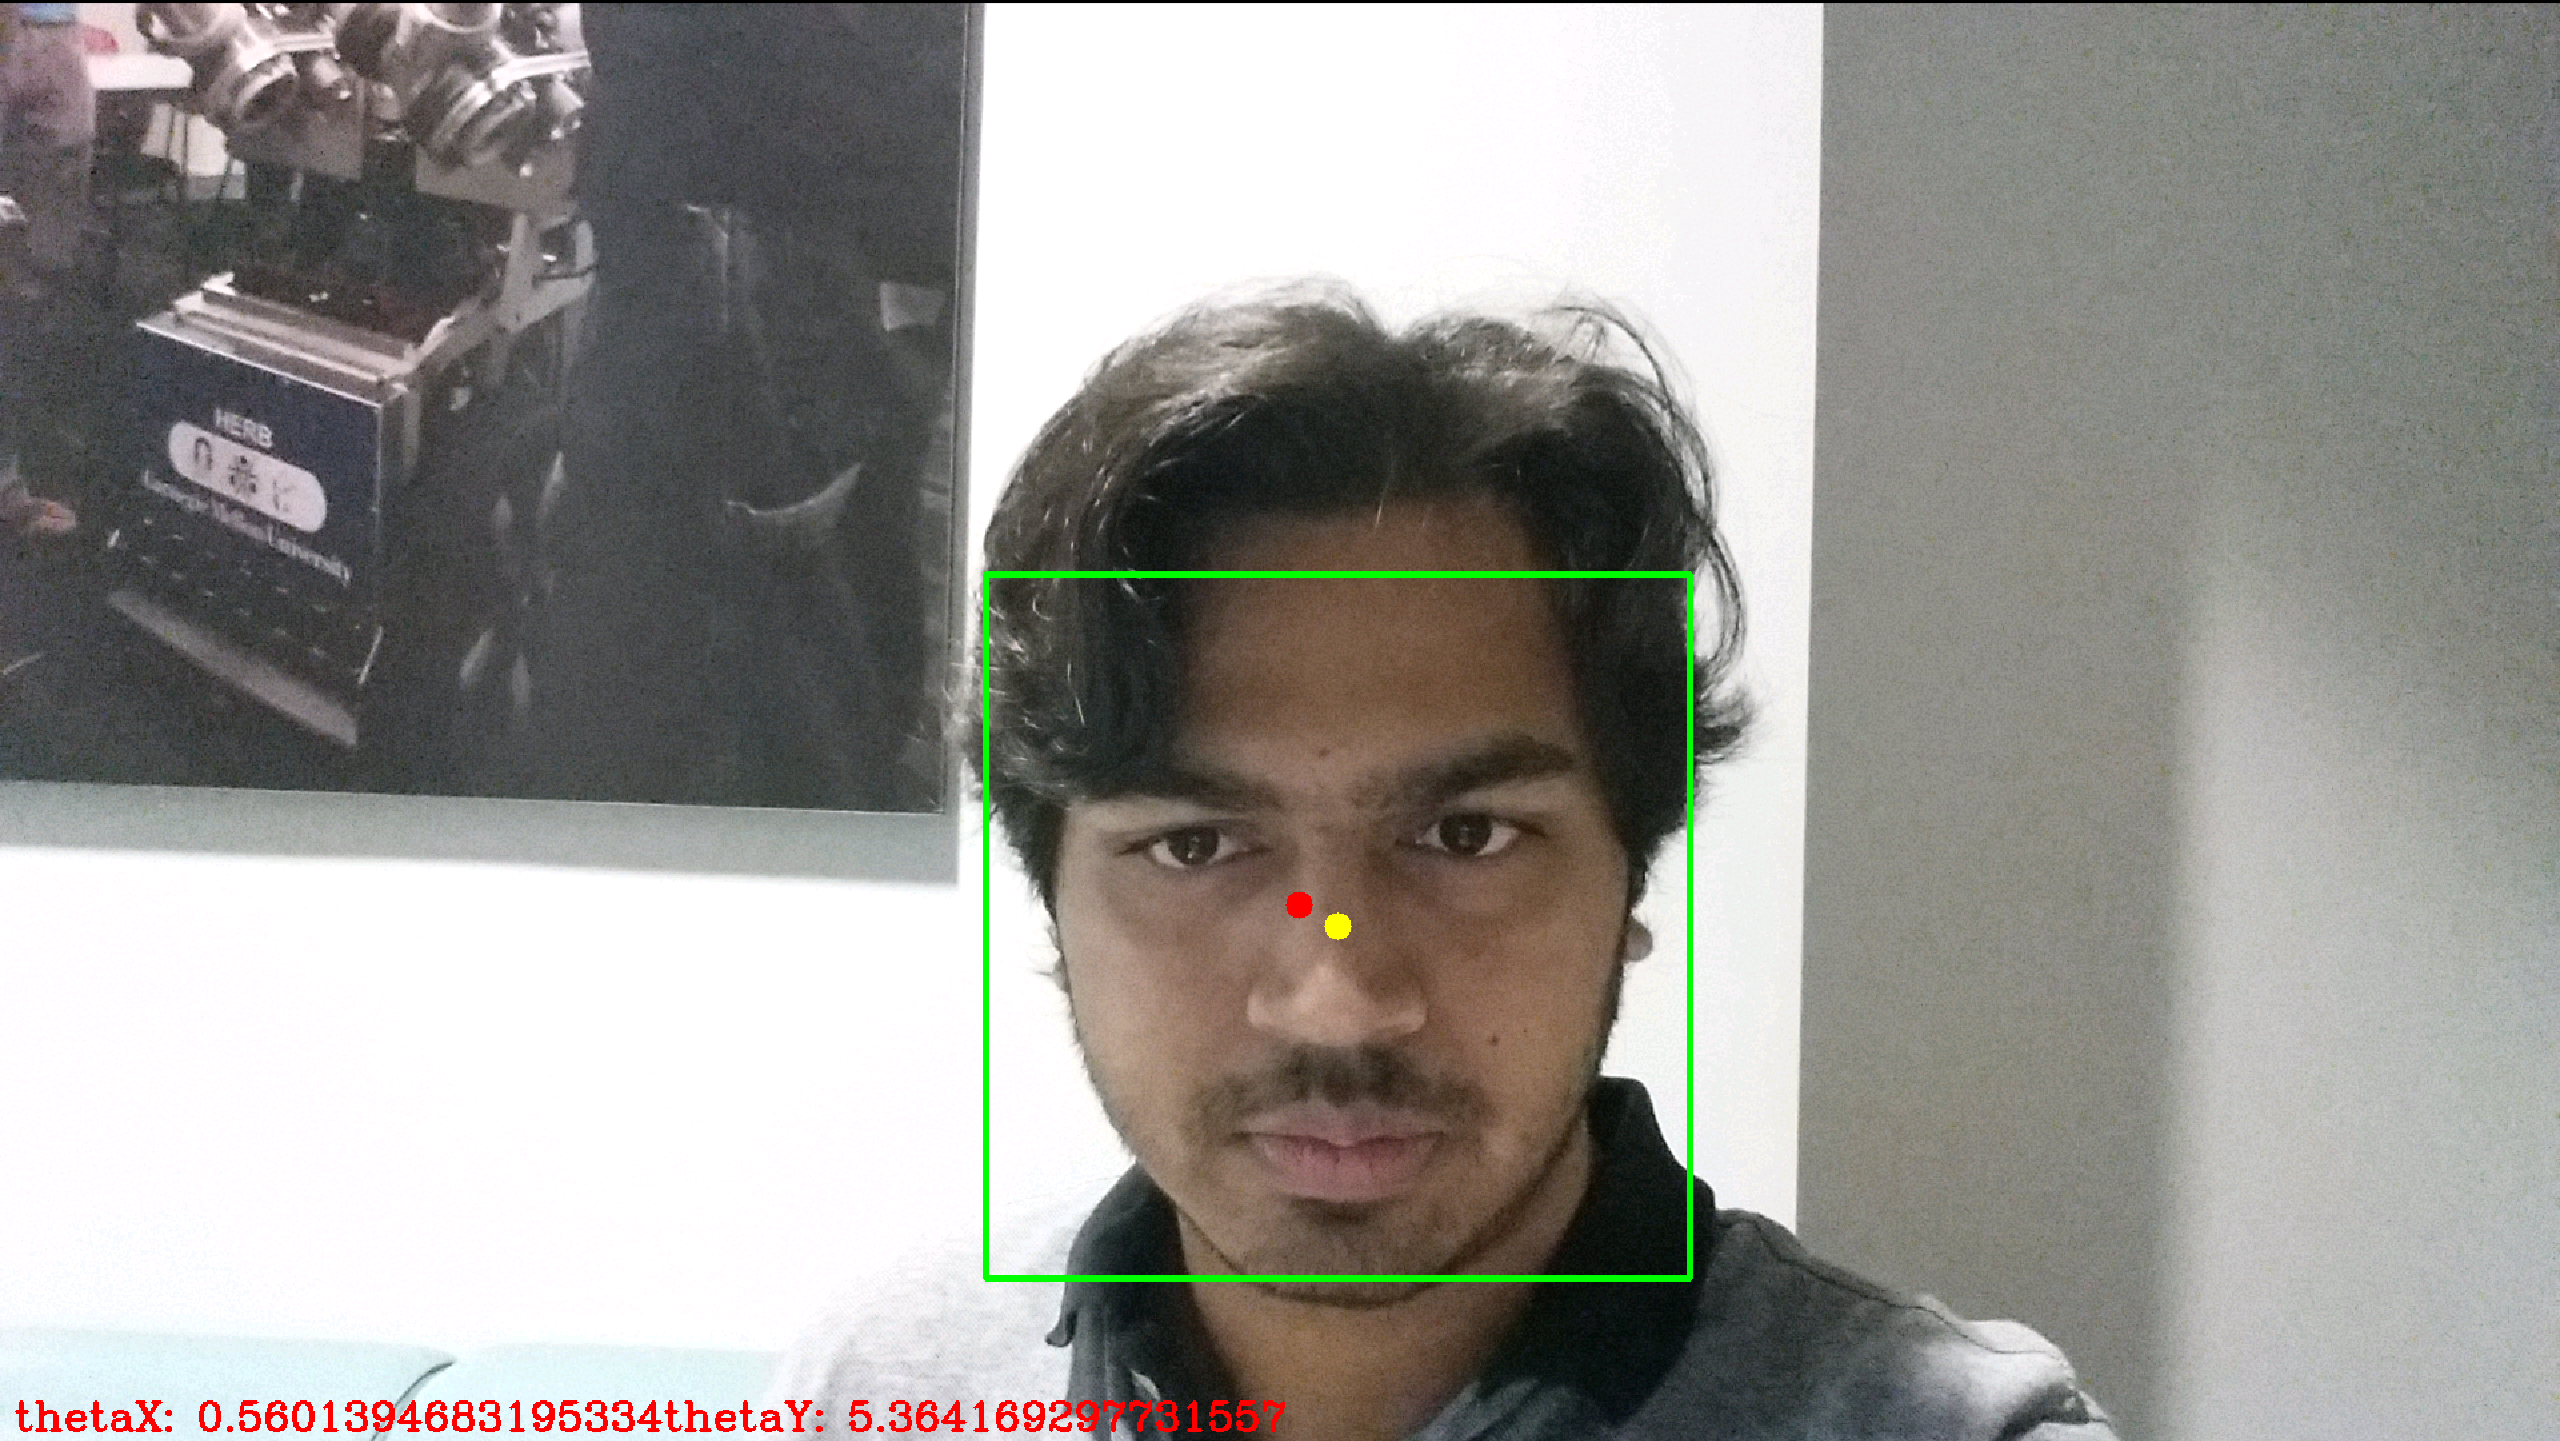
\includegraphics[scale=0.09]{jai}
\caption{Face tracking is done in 30fps with cascade classifier. $\theta_x$ and $\theta_y$ are displayed in degrees}
\end{subfigure}
\begin{subfigure}{0.5\textwidth}
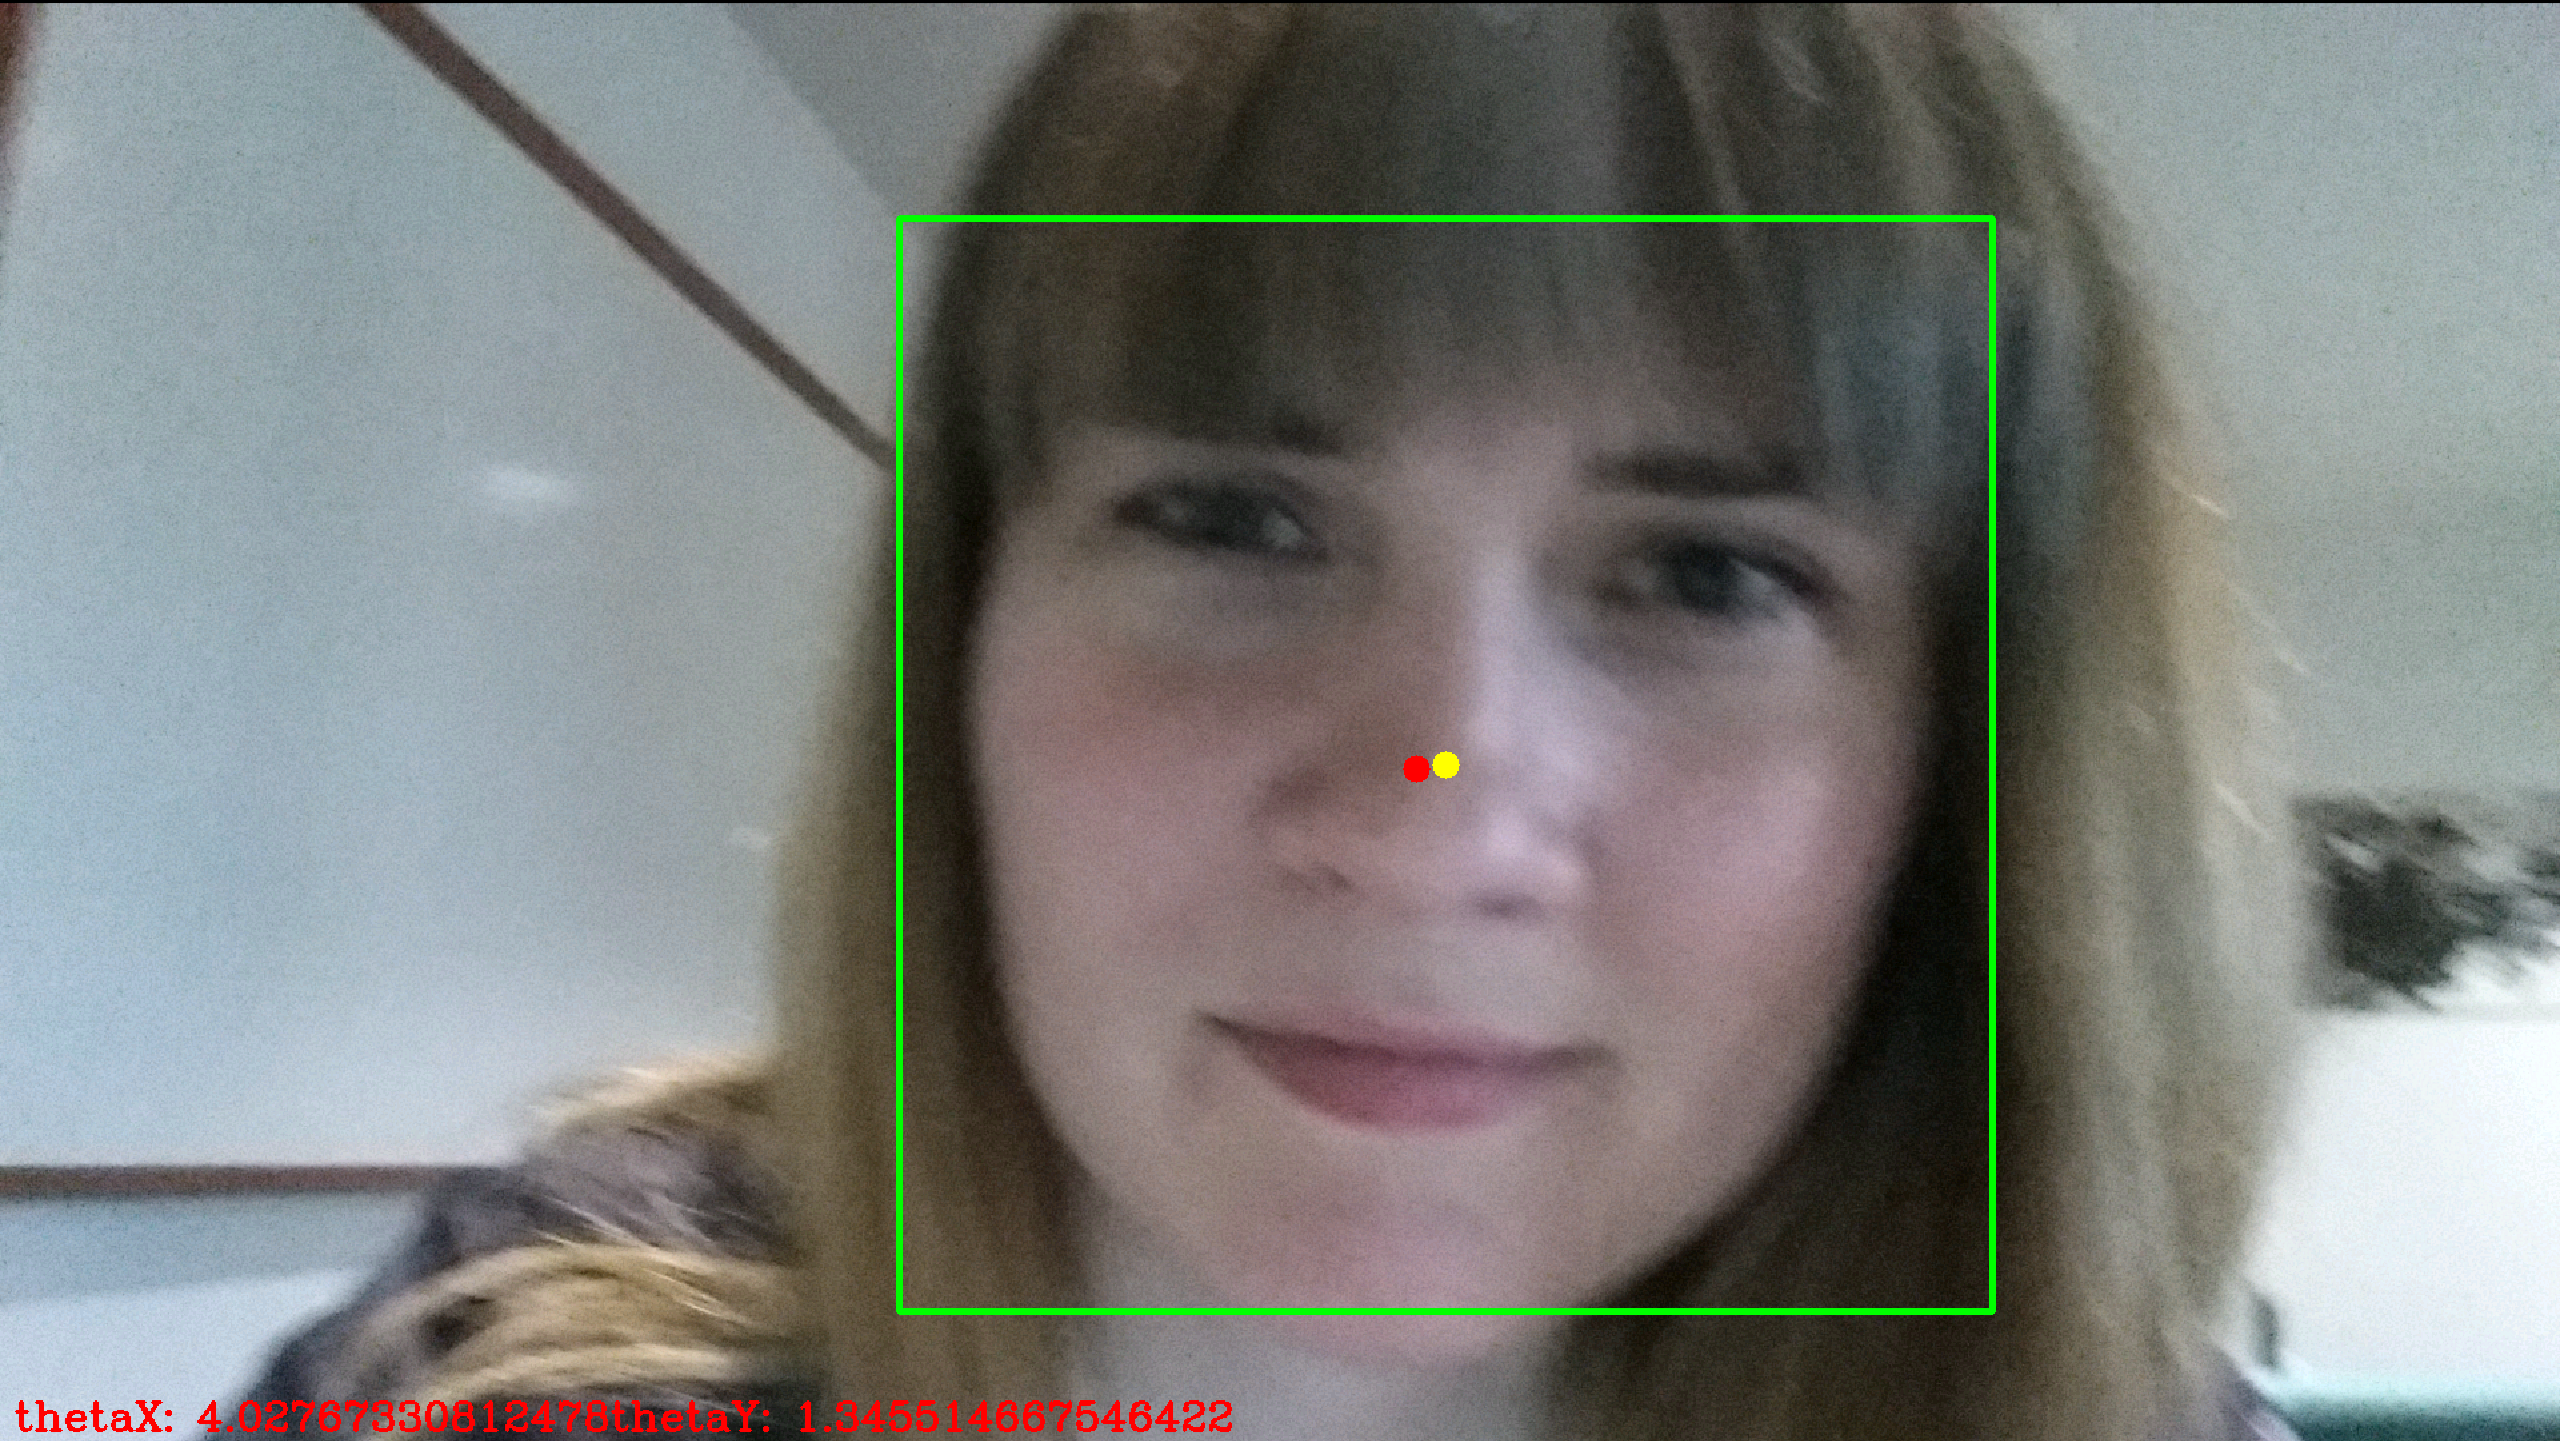
\includegraphics[scale=0.09]{jenna2}
\caption{Yellow dot shows the original centroid of face detection, red dot is the after Kalman filtering}
\end{subfigure}
\caption{Results of the working Android demo}
\label{fig:androiddemo}
\end{figure}

Figure \ref{fig:androiddemo2} is an extension of the positive parallax concept which includes both the perspective change and the 3D rendering. The perspective change is because of the change in user's angle and the 3D rendering adds the depth perception to the perspective change making the system much more immersive. 


\begin{figure}[!htbp]
\begin{subfigure}{0.5\textwidth}
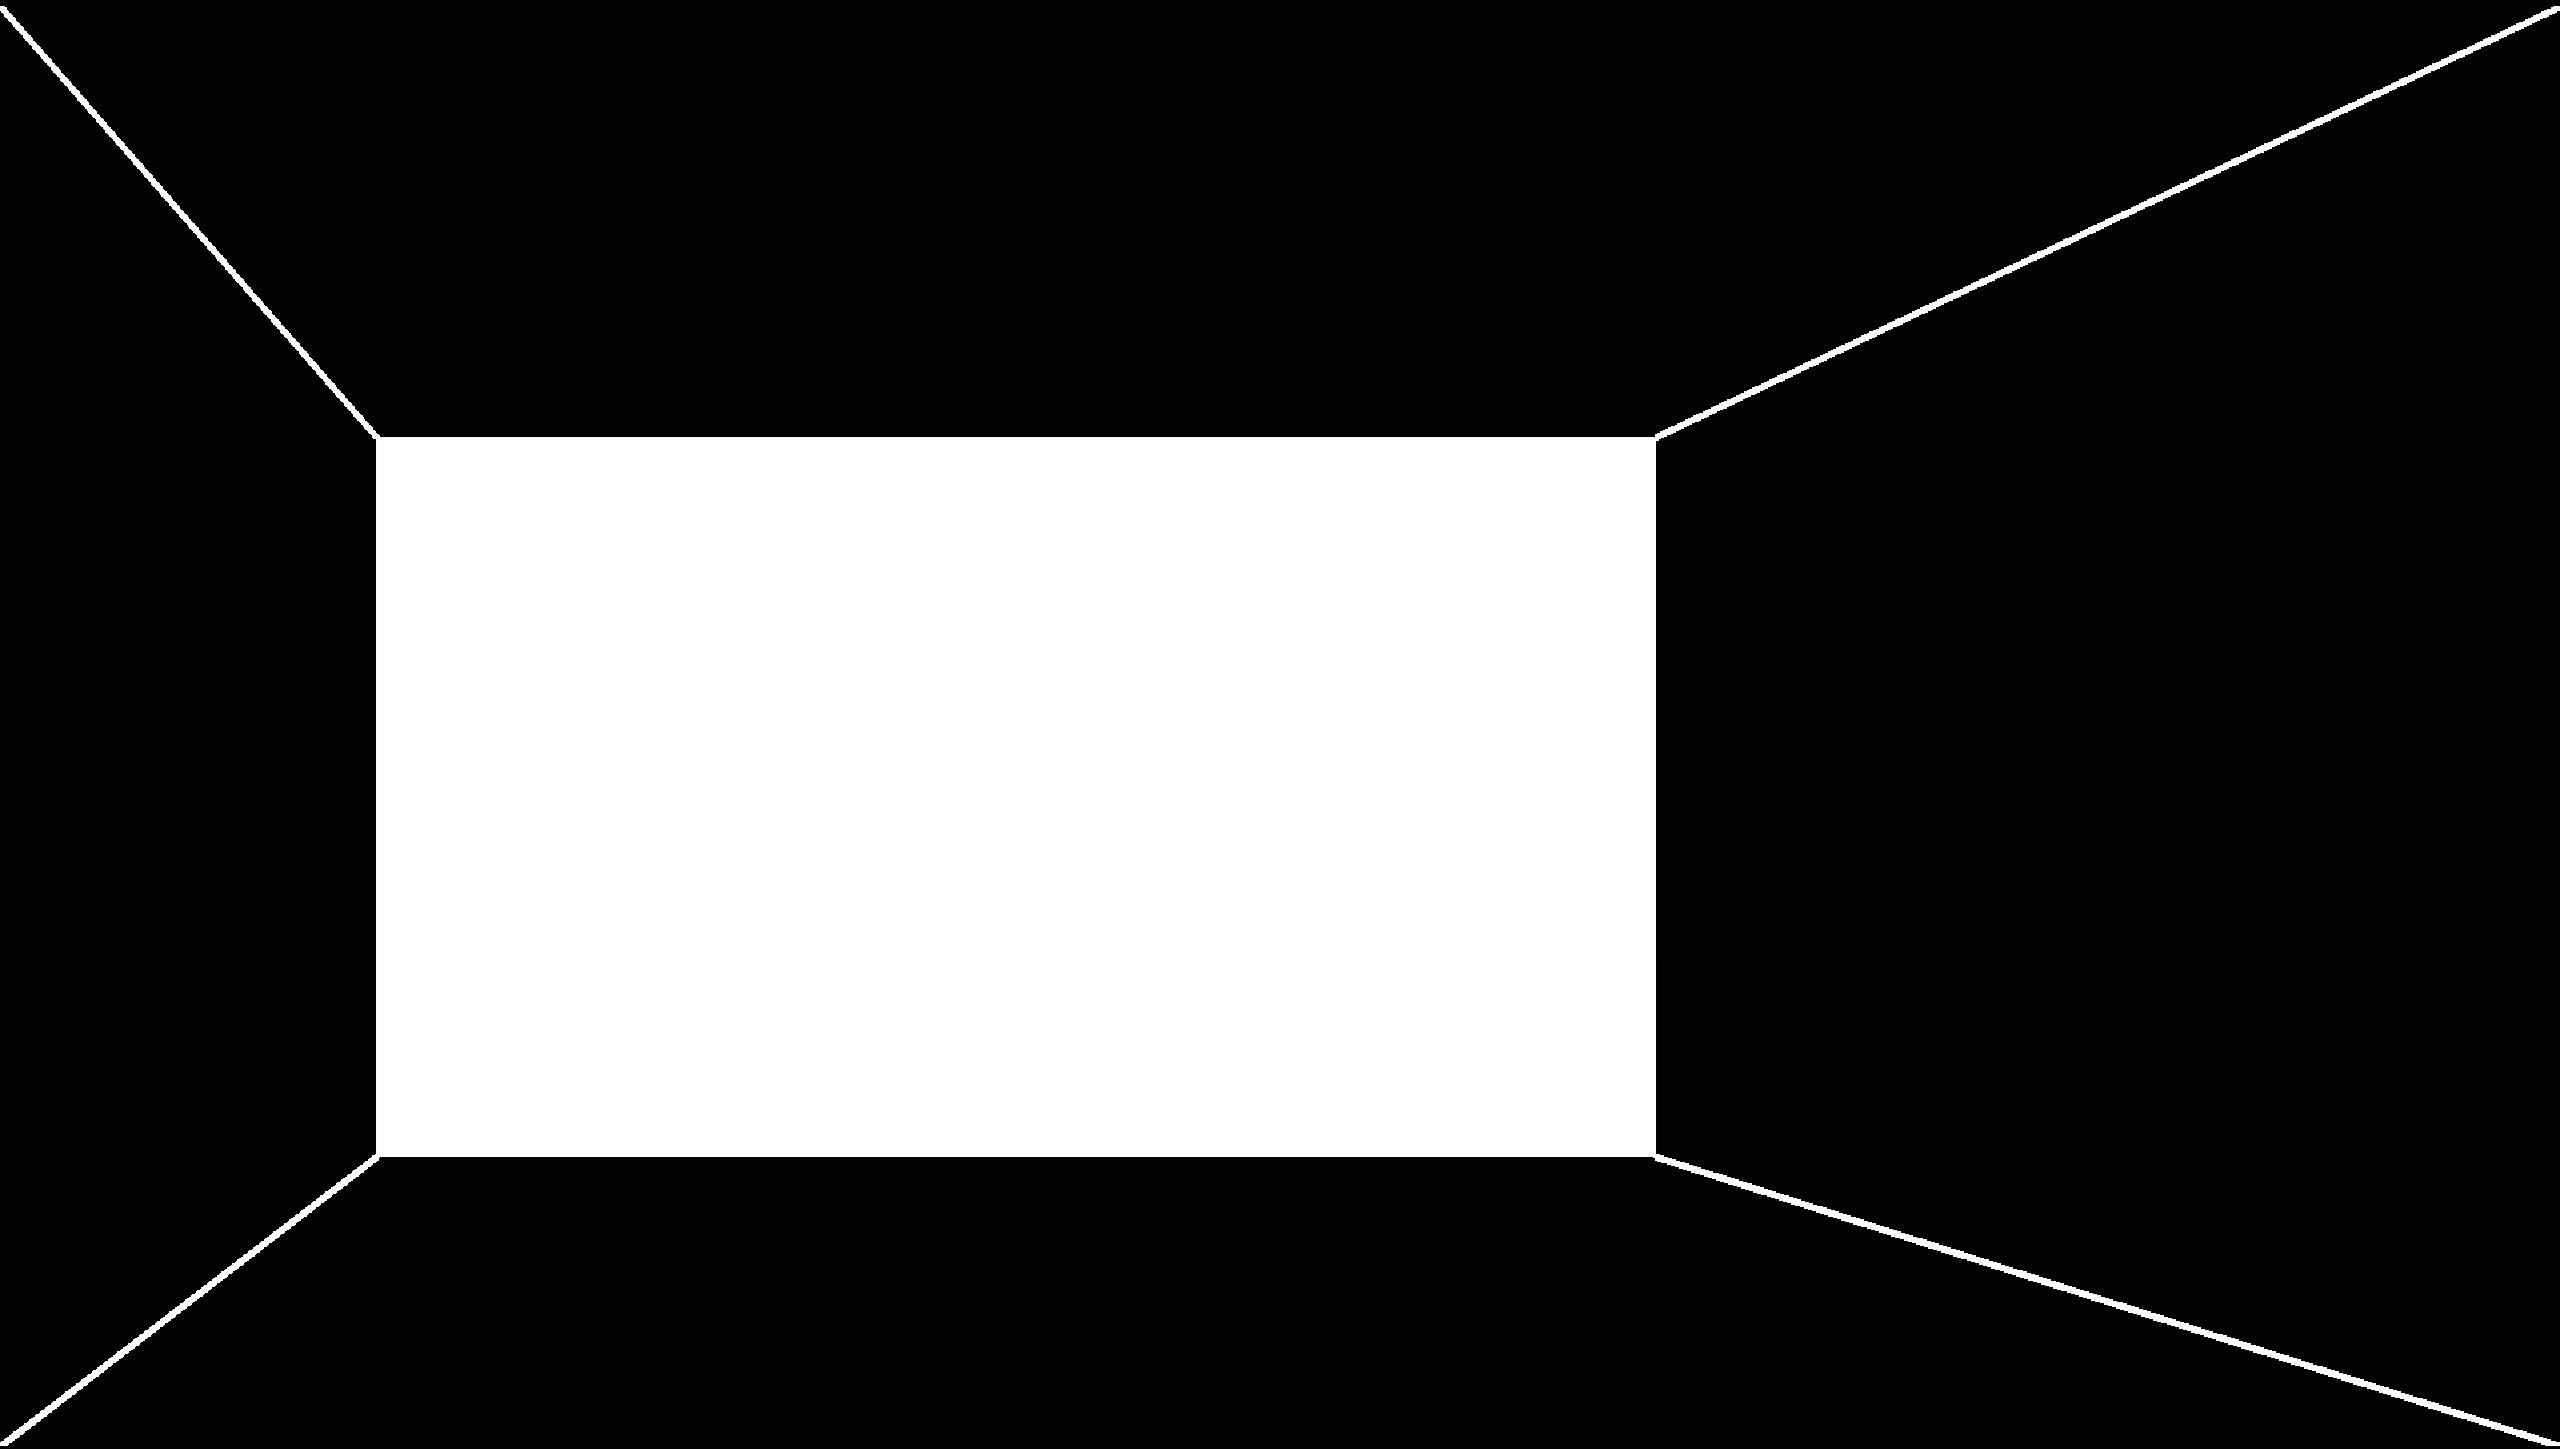
\includegraphics[scale=0.09]{3dperspective_user_left}
\caption{UI change when the user views the tablet from left}
\end{subfigure}
\begin{subfigure}{0.5\textwidth}
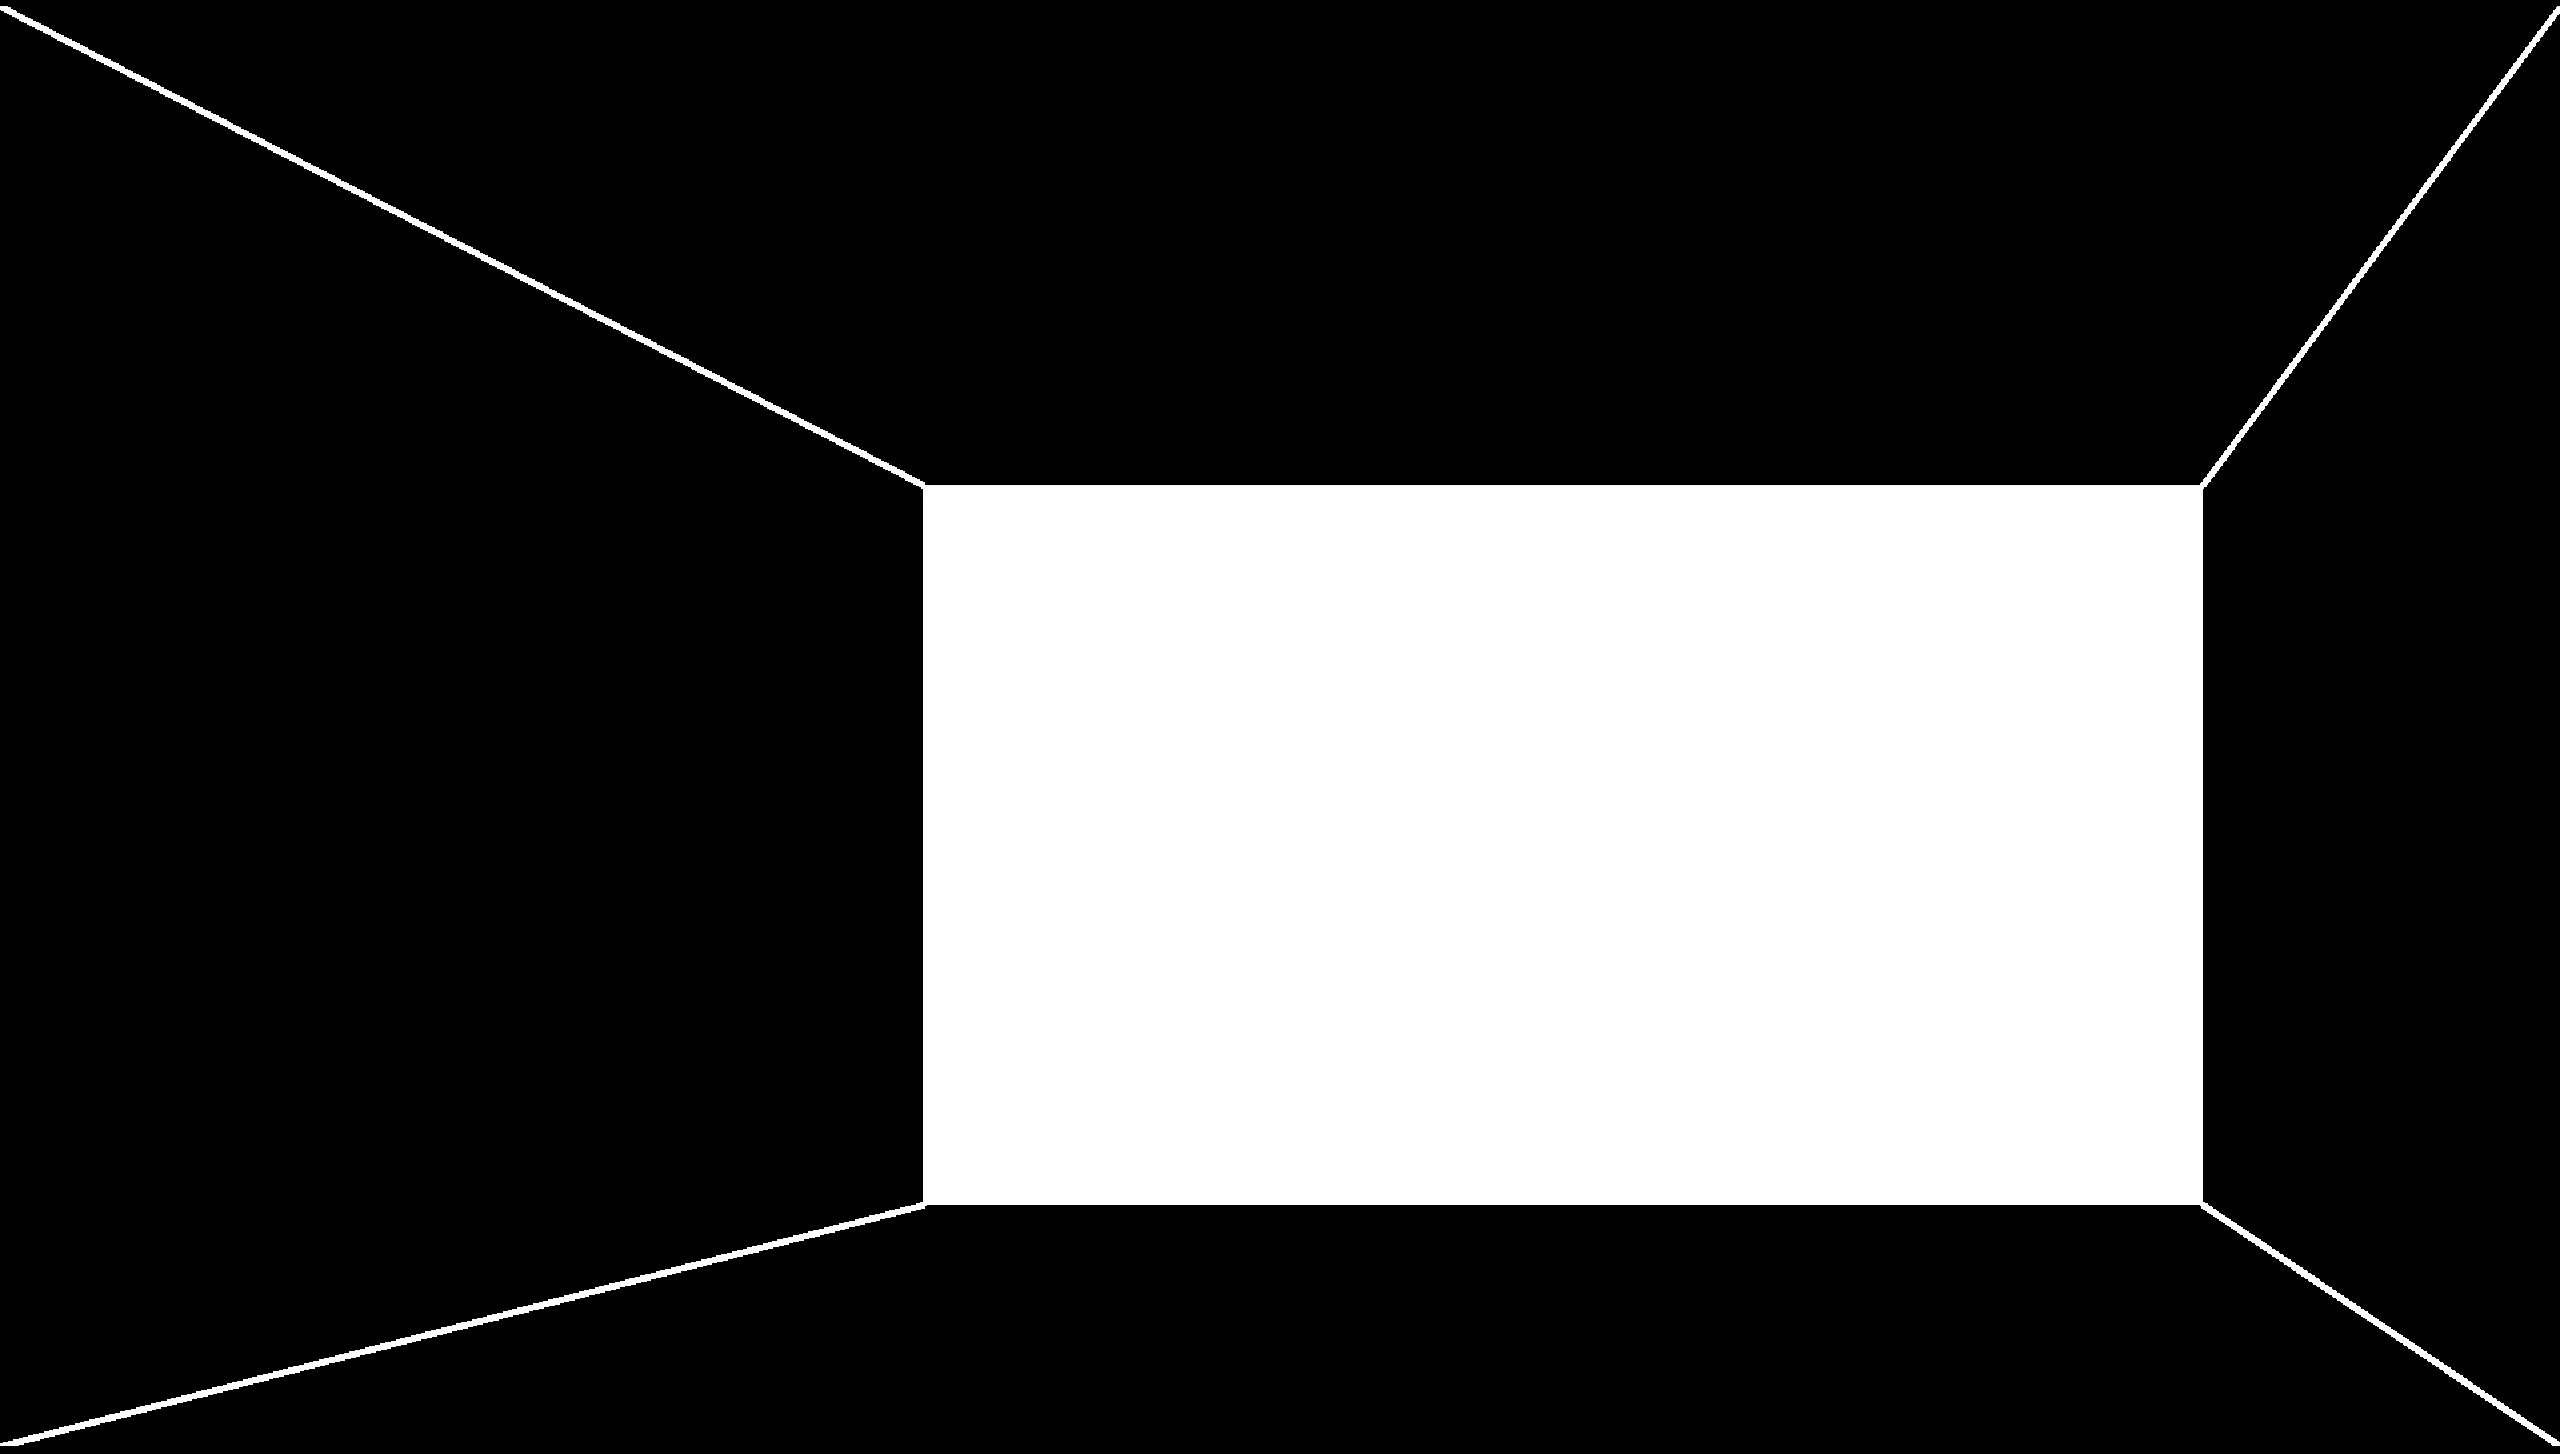
\includegraphics[scale=0.09]{3dperspective_user_right}
\caption{UI change when user views the tablet from right}
\end{subfigure}
\begin{subfigure}{0.5\textwidth}
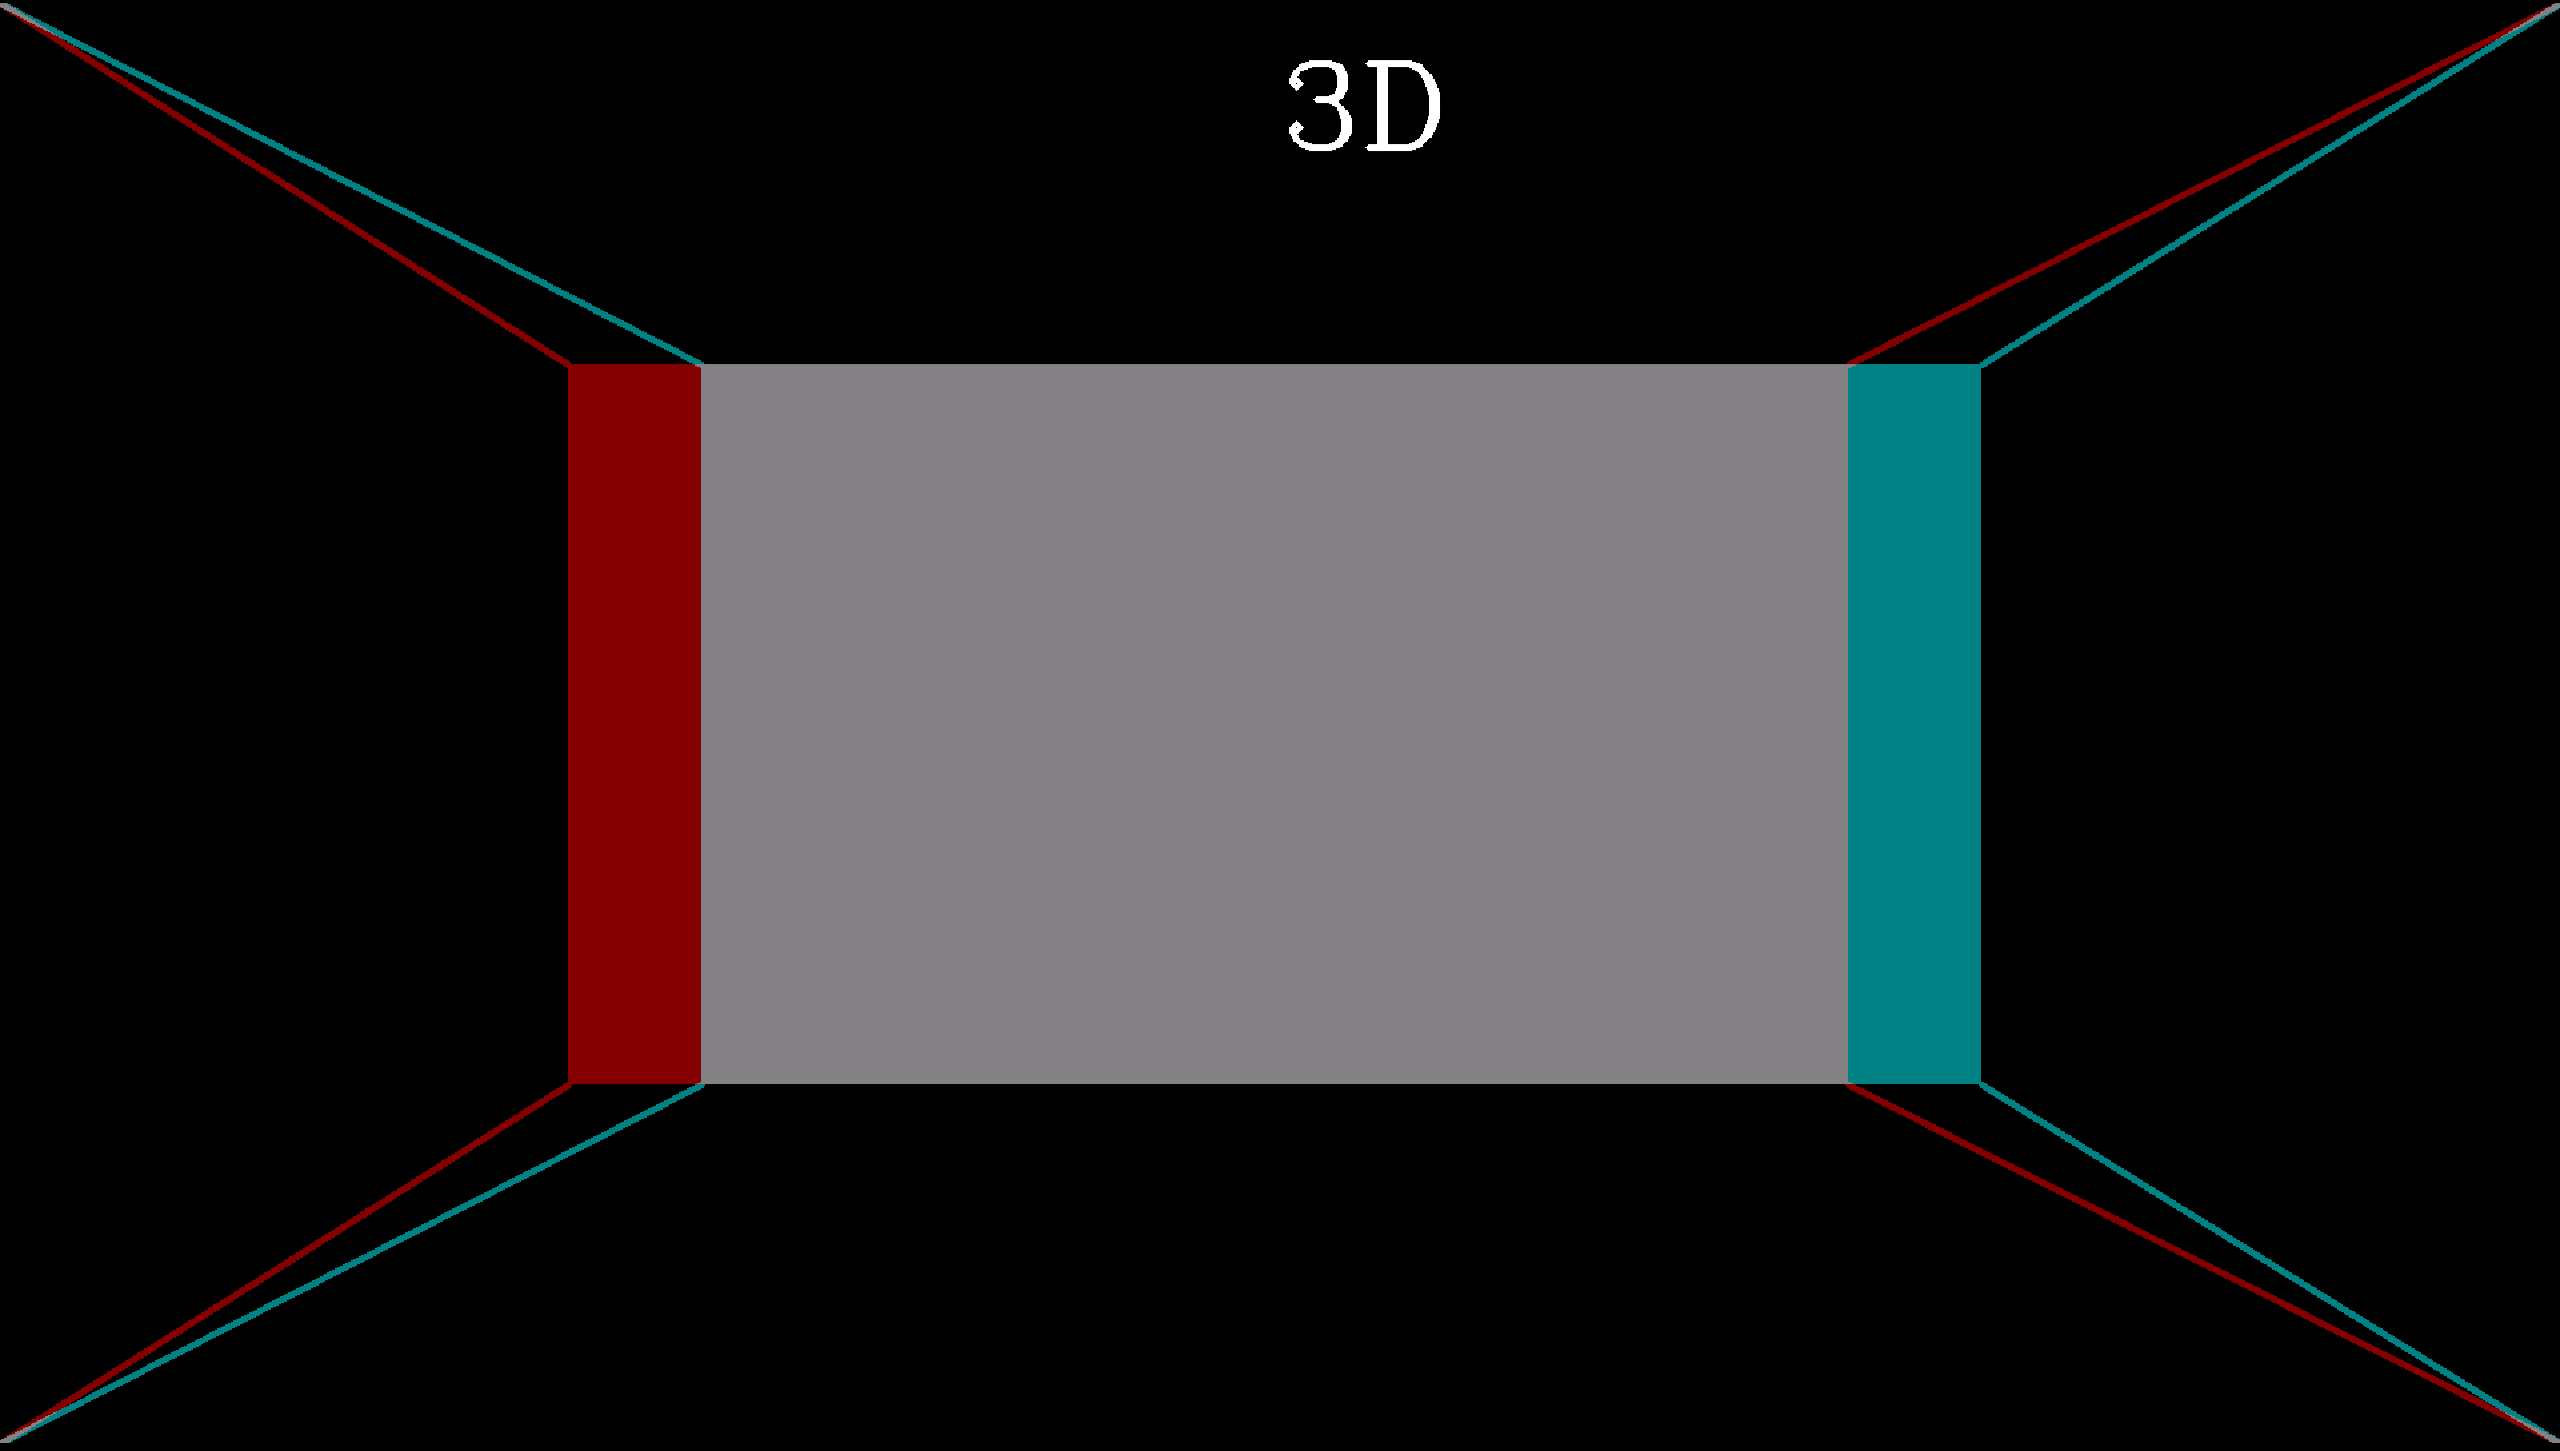
\includegraphics[scale=0.09]{anaglyph}
\end{subfigure}
\caption{More results of the working Android demo}
\label{fig:androiddemo2}
\end{figure}

\section{Conclusions}
On a whole, the face detection worked very well and we are pleased with the results after applying Kalman filtering.  This allowed for a smooth tracking of the user's face in real time. The positive parallax effects felt responsive to users we surveyed and the 3D anaglyph effect was successful.  

In the future, we would like to calculate the viewing distance of the user, so that we can scale the positive parallax effect accordingly.  When the user is far away, we would like the positive parallax effect to be deeper and more shallow when the user is closer.  In order to do this, we propose to approximate the interpupilliary distance to approximately 62-64 mm and use this as a ruler \cite{Army}.  

In addition, we would like to explore the 3D geometry between the rear-facing camera and objects of interest in the scene.  These calculations could allow for more Augmented Reality-type applications. This would allow the surrounding environment of the user to become interactive with the smart phone and could open up a new avenue of smart phone technology.
    
{\small{
\begin{thebibliography}{15}

\bibitem{Szeliski}
Szeliski, Richard. \textit{Computer Vision: Algorithms and Applications}. 1st ed. London: Springer-Verlag, 2010. Print.

\bibitem{Wikipedia}
\textit{Parallax Example}. Digital image. \textit{Wikipedia}. Wikimedia, 31 May 2006. Web. 15 Dec. 2015.

\bibitem{CSU}
Positive vs. Negative Parallax. Digital image. \textit{CSE 621 Contemporary Computer Graphics}. California State University, San Bernadina, n.d. Web. 15 Dec. 2015.

\bibitem{BusinessInsider}
Yarow, Jay. "Here's Why Apple Made That Motion-Effect For The Background Of The New IPhone Software." Business Insider. Business Insider, Inc, 25 Sept. 2013. Web. 11 Dec. 2015.

\bibitem{DigitalTrends}
Pelegrin, Williams. "Why Isn’t the Fire Phone Truly 3D? Amazon’s ‘Dynamic Perspective’ Tech Explained." \textit{Digital Trends}. Digital Trends, 18 June 2014. Web. 11 Dec. 2015.

\bibitem{Winscape}
Sevilla, Beth. "Winscape." \textit{Winscape}. Rational Craft, n.d. Web. 14 Dec. 2015.

\bibitem{TechCrunch}
Crook, Jordan. "Amazon’s Fire Phone Uses Depth And 3D Effects To Stand Out." \textit{TechCrunch}. TechCrunch, 18 June 2014. Web. 14 Dec. 2015.

\bibitem{jai}
Prakash, Jai, and Ajay Vijayvargiya. A Method for Obtaining Digital Transparency in Electronic Devices. Samsung, assignee. Patent 4506/CHE/2014. 16 Sept. 2012. Print.

\bibitem{Engaget}
Alvarez, Edgar. Dynamic Perspective. Digital image. \textit{Engaget}. AOL, 8 June 2014. Web. 15 Dec. 2015.

\bibitem{kalman}
 Kalman, R. E. "A New Approach to Linear Filtering and Prediction Problems". \textit{Journal of Basic Engineering, 1960}

\bibitem{Viola-Jones}
Viola, Paul, and Michael J. Jones. "Robust Real-Time Face Detection." \textit{International Journal of Computer Vision} 57.2 (2004): 137-54. \textit{ProQuest}. Web. 15 Dec. 2015.

\bibitem{calibration}
"Camera Calibration With OpenCV." \textit{OpenCV 3.0.0 Documentation}. Itseez, 10 Nov. 2014. Web. 15 Dec. 2015.  \url{http://docs.opencv.org/3.0-beta/doc/tutorials/calib3d/camera_calibration/camera_calibration.html}.

\bibitem{Bzarg}
Babb, Tim. "Bzarg." \textit{Bzarg}. Tim Babb, 11 Aug. 2015. Web. 16 Dec. 2015.

\bibitem{Army}
Gordon, C. C., Bradtmiller, B., Clauser, C.E., Churchill, T., McConville, J.T., Tebbetts, I., and Walker, R.A. (1989). 1987–1988 Anthropometric Survey of U.S. Army Personnel: Methods and Summary Statistics. TR-89-044. Natick MA: U.S. Army Natick Research, Development and Engineering Center.

\bibitem{Maria}
Ribeiro, Maria. "Kalman and Extended Kalman Filters: Concept, Derivation and Properties." Thesis. Institute for Systems and Robotics, 2004. Print.

% \bibitem{ArsTechnica}
% Cunningham, Andrew. "IPhone 6 and 6 Plus: In Deep with Apple’s Thinnest Phones." \textit{Ars Technica}. Conde Nast, 22 Sept. 2014. Web. 14 Dec. 2015.

% \bibitem{Gizmodo}
% Aguilar, Mario. "Here's Why the IPhone 5S Accelerometer Is So Screwed Up." \textit{Gizmodo}. Gawker Media, 16 Oct. 2013. Web. 14 Dec. 2015.

% \bibitem{Quan}
% Quan, Wei. \textit{INS/CNS/GNSS Integrated Navigation Technology}. Heidelberg: Springer, 2015. \textit{Springer Link}. Springer. Web. 14 Dec. 2015.

\endgroup
\end{document}